\documentclass{article}%
\usepackage[T1]{fontenc}%
\usepackage[utf8]{inputenc}%
\usepackage{lmodern}%
\usepackage{textcomp}%
\usepackage{lastpage}%
\usepackage{authblk}%
\usepackage{graphicx}%
%
\title{Porphyromonas gingivalis lipopolysaccharide regulates interleukin (IL){-}17 and IL{-}23 expression via SIRT1 modulation in human periodontal ligament cells}%
\author{Austin Johnson}%
\affil{Department of Orthopedic Surgery, Xinhua Hospital, Shanghai Jiaotong University, School of Medicine, Shanghai 200092, P.R. China}%
\date{01{-}01{-}2014}%
%
\begin{document}%
\normalsize%
\maketitle%
\section{Abstract}%
\label{sec:Abstract}%
Targeted Receptor Defending Embryonic Lymphocytic Phytic Cancers\newline%
ALVA BEACH, Calif. {-} Scientists at the Pacific Ocean Institute have completed an exciting discovery using sea droplets as the source of cancer cells while specifically targeting p38 signaling pathways.\newline%
In mouse models of metastatic cancers, the marine biotech researchers were able to understand that p38 is a very powerful anti{-}cancer signalling pathway, with the potential to advance cancer treatment.\newline%
P38 is a microtubule fat exoskeleton, explained Matthias Birkeland, PhD, lead author of the paper and senior author on the Pacific Ocean Institute paper. The p38 is a receptor that binds directly with multiple small proteins associated with the relevant protein{-}protein interolecular interaction pathway.\newline%
When exposed to cancer cells that had metastasized on a specific subpopulation of p38 receptors, p38 activation was reduced significantly by mTOR and IAP, Birkeland said. We knew that there were tumors that could inhibit the p38 signaling pathway  which would therefore be causing these tumors to proliferate. The virus in question was solely responsible for inhibiting p38{-} activation.\newline%
A combination of the sea droplets and peripheral vascular therapies enabled the researchers to safely sublease peripheral vascular activity from p38 activators, translating into a dramatic reduction in tumor expression. The results indicate that p38 activation can reverse the progression of cancer cells or stem cell death in marine cells, delivering a strong anti{-}cancer signal when needed most.\newline%
About Pacific Ocean Institute\newline%
Pacific Ocean Institute (PIE) is a global leader in ocean sciences and pollution control. Founded in 1961, PIE is the first ocean institute in the United States to establish a land{-}based operation. For 35 years, PIE has provided an unparalleled array of ocean science education and research programs. PIE is located at Pacific Ocean Institute, 3101 Camino Del Mar in Carlsbad, California, a Non{-}Managing Site, which emphasizes continuous improvement in environmental sustainability and demonstrates environmental stewardship. For more information, visit www.pacific{-}ocean{-}institute.org.

%
\subsection{Image Analysis}%
\label{subsec:ImageAnalysis}%


\begin{figure}[h!]%
\centering%
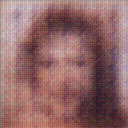
\includegraphics[width=150px]{500_fake_images/samples_5_5.png}%
\caption{A Man In A Suit And Tie Is Smiling}%
\end{figure}

%
\end{document}